It is obvious that the normal vector to the line is 
\begin{align}
\vec{n} =\myvec{2 \\ -9} -\vec{0} 
=\myvec{2 \\ -9}
\end{align}
Hence, the equation of the line is 
\begin{align}
	\myvec{2 & -9}\brak{\vec{x} - \myvec{2 \\ -9}}&= 0
	\\
	\implies 
	\myvec{2 & -9}\vec{x} &= 85
\end{align}
See 
		\figref{fig:11/10/2/15}.
	\begin{figure}[H]
		\centering
 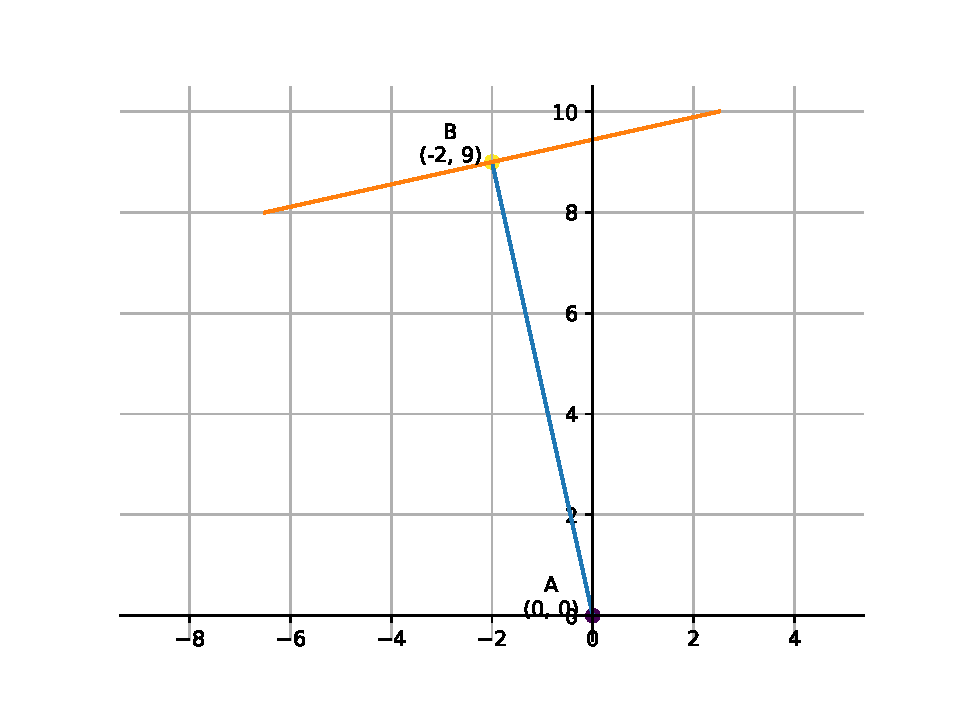
\includegraphics[width=0.75\columnwidth]{chapters/11/10/2/15/figs/fig.pdf}
		\caption{}
		\label{fig:11/10/2/15}
  	\end{figure}
